% !Mode:: "TeX:UTF-8"
%%%%%%%%%%%%%%%%%%%%%%%%%%%%%%%%%%%%%%%%%
% Thin Sectioned Essay
% LaTeX Template
% Version 1.0 (5/2/14)
%
% This template has been downloaded from:
% http://www.LaTeXTemplates.com
%
% Original Author:
% Nicolas Diaz (nsdiaz@uc.cl) with extensive modifications by:
% Vel (vel@latextemplates.com)
%
% Modifications by:
% Utopiar (Utopiar@gs.zzu.edu.cn) In ZZUNLP
%
% License:
% CC BY-NC-SA 3.0 (http://creativecommons.org/licenses/by-nc-sa/3.0/)
%
%%%%%%%%%%%%%%%%%%%%%%%%%%%%%%%%%%%%%%%%%

%----------------------------------------------------------------------------------------
%	引入支持包和文档设置
%----------------------------------------------------------------------------------------

\documentclass[a4paper, 11pt, hyperref, UTF8]{ctexart} % 字体大小 (可以设置为 10pt, 11pt or 12pt) and 纸张大小 (remove a4paper for US letter paper),汉语支持,增加hyperref可以防止生成PDF的标签乱码,若不需要生成标签,可以去掉
%\documentclass[a4paper, 11pt]{article}

\usepackage[protrusion=true,expansion=true]{microtype} % Better typography
\usepackage{graphicx} % 图片包
\usepackage{wrapfig} % 允许图片或绕

\usepackage{float} %图片位置
\usepackage{amsmath} %公式
\usepackage{bm}  %加粗
\usepackage{CJK} %字体包

\usepackage[colorlinks,linkcolor=black,anchorcolor=black,citecolor=black]{hyperref}  %超链接包

\usepackage{mathpazo} % 使用Palatino字体
\usepackage[T1]{fontenc} % Required for accented characters
\linespread{1.05} % 更改行间距, Palatino字体默认改行最佳

\makeatletter
%\renewcommand\@biblabel[1]{\textbf{#1.}} % 更换引用序号'[1]' 为'1.'
\renewcommand{\@listI}{\itemsep=0pt} % 减少逐项列举项目之间的空间,并列举环境和参考书目

\renewcommand{\maketitle}{ % 自定义标题 - 在这里并不修改标题和作者的名字
\begin{flushleft} % 左/右对齐
{\LARGE\@title} % 加大标题字体

\vspace{50pt} % 标题和作者间的间距

{\large\@author} % 作者名格式
\\\@date % Date

\vspace{40pt} % 作者和摘要的距离
\end{flushleft}
}

%----------------------------------------------------------------------------------------
%	TITLE
%----------------------------------------------------------------------------------------

%TODO
\title{\textbf{Title}\\ % Title
SubTitle} % Subtitle

%TODO
\author{\textsc{Author} % Author
\\{\textit{Institution}}} % Institution

\date{\today} % Date

%----------------------------------------------------------------------------------------

\begin{document}
\maketitle % Print the title section
text\cite{rogers2011first} text\cite{harrington2012machine} %添加引用
%----------------------------------------------------------------------------------------
%	ABSTRACT AND KEYWORDS
%----------------------------------------------------------------------------------------

%\renewcommand{\abstractname}{Summary} % Uncomment to change the name of the abstract to something else

\begin{abstract}
此处为摘要部分……

\begin{enumerate}
\item 条目1
\item 条目2
\end{enumerate}

\end{abstract}

\hspace*{3,6mm}\textit{Keywords:} 关键字 % Keywords

\vspace{30pt} % Some vertical space between the abstract and first section

%----------------------------------------------------------------------------------------
%	ESSAY BODY
%----------------------------------------------------------------------------------------

\section{第一部分}

第一部分
%--------------------------------------------------------------------------------------------
\subsection{第一节}
\paragraph{测试}测试
%------------------------------------------------

\subsection{第二节}

%-------------------------------------------------------------------------------------------
%插入图片
%------------------------------------------------------------------------------------------

\begin{figure}[H]
\centering
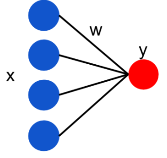
\includegraphics[width=0.38\textwidth,height=0.38\textwidth]{1.png}
\caption{线性回归}
\end{figure}
\paragraph{测试}测试


%------------------------------------------------


\subsection{第三节}

%--------------------------------------------------
%插入图片
%--------------------------------------------------

\begin{figure}[H]
\centering
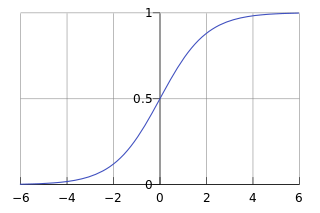
\includegraphics[width=0.38\textwidth,height=0.38\textwidth]{2.png}
\caption{Logistic方程}
\end{figure}

\paragraph{测试}测试

%---------------------------------------------------

\section{第二部分}

\paragraph{测试}测试

\subsection{第一节}

\paragraph{测试}测试

%-----------------------------
%插入公式
%-----------------------------

$$ L=\prod_{i=1}^{N}{[P(Y=1|x_i)]^{y_i} [P(Y=0|x_i)]^{1-y_i}} $$
有连乘,这个好办,取对数就OK:

\begin{align*}
 L(w) &= \sum _{i=1} ^{N} {y^i log(P(Y=1|x_i)) + (1-y^i)log(P(Y=0|x_i))} \\
      &= \sum _{i=1} ^{N} {y^i log(P(Y=1|x_i)) + log(P(Y=0|x_i)) - y^ilog(P(Y=0|x_i))} \\
      &= \sum _{i=1} ^{N} {y^i log\frac{P(Y=1|x_i)} {P(Y=0|x_i)} + log(P(Y=0|x_i))} \\
\end{align*}

%--------------------------------------
%插入图表
%--------------------------------------

\begin{center}
\begin{tabular}{c|c}
\hline
$f(w)$                 & $\frac{\partial{f}}{\partial{w}}$   \\
\hline
$\bm{w}^T\bm{x}$       & $\bm{x}$                            \\
%\hline
$\bm{x}^T\bm{w}$       & $\bm{x}$                            \\
%\hline
$\bm{w}^T\bm{w}$       & $2\bm{w}$                           \\
%\hline
$\bm{x}^T\bm{C}\bm{w}$ & $2\bm{Cx}$                          \\
\hline
\end{tabular}
\end{center}



%----------------------------------------------------------------------------------------
%	BIBLIOGRAPHY
%----------------------------------------------------------------------------------------

%\begin{thebibliography}{0}

%\bibitem{Harrington2012}
%Harrington, Peter. \emph{Machine Learning in Action}. Manning Publications Co., 2012.

%\bibitem{Rogers2011}
%Rogers, Simon, and Mark Girolami. \emph{A first course in machine learning}. CRC Press, 2011.

%\bibitem{zouxy092014}
%zouxy09. \emph{\href{http://blog.csdn.net/zouxy09/article/details/20319673}{机器学习算法与Python实践之(七)逻辑回归(Logistic Regression)}}.  CSDN, 2014.

%\bibitem{Su2011}
%苏冉旭. \emph{\href{http://hi.baidu.com/hehehehello/item/40025c33d7d9b7b9633aff87}{逻辑回归概述}}. 百度, 2011.

%\bibitem{daniel-D2013}
%daniel-D.  \emph{\href{http://www.cnblogs.com/daniel-D/archive/2013/05/30/3109276.html}{Logistic Regression 之基础知识准备}}. cnblog, 2013.
%\end{thebibliography}

%-------------------------------------------------------------------------------------------------------
%使用bibtex文件
%-------------------------------------------------------------------------------------------------------

\bibliographystyle{unsrt}

\bibliography{Rogers}
%-------------------------------rogers2011first---------------------------------------------------------
\end{document}
